% Options for packages loaded elsewhere
\PassOptionsToPackage{unicode}{hyperref}
\PassOptionsToPackage{hyphens}{url}
%
\documentclass[
  man,floatsintext]{apa6}
\usepackage{amsmath,amssymb}
\usepackage{lmodern}
\usepackage{iftex}
\ifPDFTeX
  \usepackage[T1]{fontenc}
  \usepackage[utf8]{inputenc}
  \usepackage{textcomp} % provide euro and other symbols
\else % if luatex or xetex
  \usepackage{unicode-math}
  \defaultfontfeatures{Scale=MatchLowercase}
  \defaultfontfeatures[\rmfamily]{Ligatures=TeX,Scale=1}
\fi
% Use upquote if available, for straight quotes in verbatim environments
\IfFileExists{upquote.sty}{\usepackage{upquote}}{}
\IfFileExists{microtype.sty}{% use microtype if available
  \usepackage[]{microtype}
  \UseMicrotypeSet[protrusion]{basicmath} % disable protrusion for tt fonts
}{}
\makeatletter
\@ifundefined{KOMAClassName}{% if non-KOMA class
  \IfFileExists{parskip.sty}{%
    \usepackage{parskip}
  }{% else
    \setlength{\parindent}{0pt}
    \setlength{\parskip}{6pt plus 2pt minus 1pt}}
}{% if KOMA class
  \KOMAoptions{parskip=half}}
\makeatother
\usepackage{xcolor}
\usepackage{graphicx}
\makeatletter
\def\maxwidth{\ifdim\Gin@nat@width>\linewidth\linewidth\else\Gin@nat@width\fi}
\def\maxheight{\ifdim\Gin@nat@height>\textheight\textheight\else\Gin@nat@height\fi}
\makeatother
% Scale images if necessary, so that they will not overflow the page
% margins by default, and it is still possible to overwrite the defaults
% using explicit options in \includegraphics[width, height, ...]{}
\setkeys{Gin}{width=\maxwidth,height=\maxheight,keepaspectratio}
% Set default figure placement to htbp
\makeatletter
\def\fps@figure{htbp}
\makeatother
\setlength{\emergencystretch}{3em} % prevent overfull lines
\providecommand{\tightlist}{%
  \setlength{\itemsep}{0pt}\setlength{\parskip}{0pt}}
\setcounter{secnumdepth}{-\maxdimen} % remove section numbering
% Make \paragraph and \subparagraph free-standing
\ifx\paragraph\undefined\else
  \let\oldparagraph\paragraph
  \renewcommand{\paragraph}[1]{\oldparagraph{#1}\mbox{}}
\fi
\ifx\subparagraph\undefined\else
  \let\oldsubparagraph\subparagraph
  \renewcommand{\subparagraph}[1]{\oldsubparagraph{#1}\mbox{}}
\fi
\newlength{\cslhangindent}
\setlength{\cslhangindent}{1.5em}
\newlength{\csllabelwidth}
\setlength{\csllabelwidth}{3em}
\newlength{\cslentryspacingunit} % times entry-spacing
\setlength{\cslentryspacingunit}{\parskip}
\newenvironment{CSLReferences}[2] % #1 hanging-ident, #2 entry spacing
 {% don't indent paragraphs
  \setlength{\parindent}{0pt}
  % turn on hanging indent if param 1 is 1
  \ifodd #1
  \let\oldpar\par
  \def\par{\hangindent=\cslhangindent\oldpar}
  \fi
  % set entry spacing
  \setlength{\parskip}{#2\cslentryspacingunit}
 }%
 {}
\usepackage{calc}
\newcommand{\CSLBlock}[1]{#1\hfill\break}
\newcommand{\CSLLeftMargin}[1]{\parbox[t]{\csllabelwidth}{#1}}
\newcommand{\CSLRightInline}[1]{\parbox[t]{\linewidth - \csllabelwidth}{#1}\break}
\newcommand{\CSLIndent}[1]{\hspace{\cslhangindent}#1}
\ifLuaTeX
\usepackage[bidi=basic]{babel}
\else
\usepackage[bidi=default]{babel}
\fi
\babelprovide[main,import]{english}
% get rid of language-specific shorthands (see #6817):
\let\LanguageShortHands\languageshorthands
\def\languageshorthands#1{}
% Manuscript styling
\usepackage{upgreek}
\captionsetup{font=singlespacing,justification=justified}

% Table formatting
\usepackage{longtable}
\usepackage{lscape}
% \usepackage[counterclockwise]{rotating}   % Landscape page setup for large tables
\usepackage{multirow}		% Table styling
\usepackage{tabularx}		% Control Column width
\usepackage[flushleft]{threeparttable}	% Allows for three part tables with a specified notes section
\usepackage{threeparttablex}            % Lets threeparttable work with longtable

% Create new environments so endfloat can handle them
% \newenvironment{ltable}
%   {\begin{landscape}\centering\begin{threeparttable}}
%   {\end{threeparttable}\end{landscape}}
\newenvironment{lltable}{\begin{landscape}\centering\begin{ThreePartTable}}{\end{ThreePartTable}\end{landscape}}

% Enables adjusting longtable caption width to table width
% Solution found at http://golatex.de/longtable-mit-caption-so-breit-wie-die-tabelle-t15767.html
\makeatletter
\newcommand\LastLTentrywidth{1em}
\newlength\longtablewidth
\setlength{\longtablewidth}{1in}
\newcommand{\getlongtablewidth}{\begingroup \ifcsname LT@\roman{LT@tables}\endcsname \global\longtablewidth=0pt \renewcommand{\LT@entry}[2]{\global\advance\longtablewidth by ##2\relax\gdef\LastLTentrywidth{##2}}\@nameuse{LT@\roman{LT@tables}} \fi \endgroup}

% \setlength{\parindent}{0.5in}
% \setlength{\parskip}{0pt plus 0pt minus 0pt}

% Overwrite redefinition of paragraph and subparagraph by the default LaTeX template
% See https://github.com/crsh/papaja/issues/292
\makeatletter
\renewcommand{\paragraph}{\@startsection{paragraph}{4}{\parindent}%
  {0\baselineskip \@plus 0.2ex \@minus 0.2ex}%
  {-1em}%
  {\normalfont\normalsize\bfseries\itshape\typesectitle}}

\renewcommand{\subparagraph}[1]{\@startsection{subparagraph}{5}{1em}%
  {0\baselineskip \@plus 0.2ex \@minus 0.2ex}%
  {-\z@\relax}%
  {\normalfont\normalsize\itshape\hspace{\parindent}{#1}\textit{\addperi}}{\relax}}
\makeatother

% \usepackage{etoolbox}
\makeatletter
\patchcmd{\HyOrg@maketitle}
  {\section{\normalfont\normalsize\abstractname}}
  {\section*{\normalfont\normalsize\abstractname}}
  {}{\typeout{Failed to patch abstract.}}
\patchcmd{\HyOrg@maketitle}
  {\section{\protect\normalfont{\@title}}}
  {\section*{\protect\normalfont{\@title}}}
  {}{\typeout{Failed to patch title.}}
\makeatother

\usepackage{xpatch}
\makeatletter
\xapptocmd\appendix
  {\xapptocmd\section
    {\addcontentsline{toc}{section}{\appendixname\ifoneappendix\else~\theappendix\fi\\: #1}}
    {}{\InnerPatchFailed}%
  }
{}{\PatchFailed}
\keywords{visual illusions, illusion game, Pyllusion, personality, general factor\newline\indent Word count: 4085}
\usepackage{lineno}

\linenumbers
\usepackage{csquotes}
\usepackage[titles]{tocloft}
\cftpagenumbersoff{figure}
\renewcommand{\cftfigpresnum}{\itshape\figurename\enspace}
\renewcommand{\cftfigaftersnum}{.\space}
\setlength{\cftfigindent}{0pt}
\setlength{\cftafterloftitleskip}{0pt}
\settowidth{\cftfignumwidth}{Figure 10.\qquad}
\usepackage[labelfont=bf, font={scriptsize, color=gray}]{caption}
\ifLuaTeX
  \usepackage{selnolig}  % disable illegal ligatures
\fi
\IfFileExists{bookmark.sty}{\usepackage{bookmark}}{\usepackage{hyperref}}
\IfFileExists{xurl.sty}{\usepackage{xurl}}{} % add URL line breaks if available
\urlstyle{same} % disable monospaced font for URLs
\hypersetup{
  pdftitle={Adaptation of the PHQ-4 Short Screening for Depression and Anxiety to increase its Sensitivity to Subclinical Variability},
  pdfauthor={Dominique Makowski1, An Shu Te1, \& S.H. Annabel Chen1, 2, 3, 4},
  pdflang={en-EN},
  pdfkeywords={visual illusions, illusion game, Pyllusion, personality, general factor},
  hidelinks,
  pdfcreator={LaTeX via pandoc}}

\title{\textbf{Adaptation of the PHQ-4 Short Screening for Depression and Anxiety to increase its Sensitivity to Subclinical Variability}}
\author{Dominique Makowski\textsuperscript{1}, An Shu Te\textsuperscript{1}, \& S.H. Annabel Chen\textsuperscript{1, 2, 3, 4}}
\date{}


\shorttitle{PHQ-4R}

\authornote{

The authors made the following contributions. Dominique Makowski: Conceptualization, Data curation, Formal Analysis, Funding acquisition, Investigation, Methodology, Project administration, Resources, Software, Supervision, Validation, Visualization, Writing -- original draft; An Shu Te: Project administration, Resources, Investigation, Writing -- original draft; S.H. Annabel Chen: Project administration, Supervision, Writing -- review \& editing.

Correspondence concerning this article should be addressed to Dominique Makowski, HSS 04-18, 48 Nanyang Avenue, Singapore. E-mail: \href{mailto:dom.makowski@gmail.com}{\nolinkurl{dom.makowski@gmail.com}}

}

\affiliation{\vspace{0.5cm}\textsuperscript{1} School of Social Sciences, Nanyang Technological University, Singapore\\\textsuperscript{2} LKC Medicine, Nanyang Technological University, Singapore\\\textsuperscript{3} National Institute of Education, Singapore\\\textsuperscript{4} Centre for Research and Development in Learning, Nanyang Technological University, Singapore}

\abstract{%
Something something

\textbf{Significance Statement}. Developing reliable and sensitive instruments for mood disorders screening is critical in a global context marked by international crises (pandemics, wars), where more and more surveys as done online. In this study, we show that a small modification to the widely used PHQ-4 scale (adding the ``Once or twice'' response option) can increase its ability to capture the mild fluctuations prevalent in subclinical samples.
}



\begin{document}
\maketitle

\hypertarget{introduction}{%
\section{Introduction}\label{introduction}}

The Patient Health Questionnaire-4 (PHQ-4) is an ultra brief measurement of core signs of depression and anxiety (Kroenke et al., 2009). It consists of two items for depression (PHQ--2) and anxiety (GAD--2), each corresponding to DSM-IV Diagnostic Criterion A symptoms for major depressive disorder (MDD) and generalized anxiety disorder (GAD). It has been validated across many languages and samples Materu et al. (2020), becoming one of the most popular screening instrument (Maurer et al., 2018).

While the scale has been validated and used in the general population Hajek \& König (2020), its initial purpose was to reliably discriminate and identify potential MDD/GAD patients. This diagnostic and discriminative goal materializes in the scale's design and the existence of categorical cut-offs. However, it might not be best suited to capture subclinical variability. In particular, the gap between the two lowest possible answers, ``Not at all'' and ``Several days'', is quite large and leaves out the possibility of more subtle occurrences. While this is not necessarily an issue in clinical and diagnostic contexts, it might lead to a sub-optimal discrimination on the lower end of the spectrum, important for instance in the context of variability quantifications. The goal of this study is to increase, with minimal changes to the scale, the sensitivity to very mild mood alterations.

\hypertarget{methods}{%
\section{Methods}\label{methods}}

\hypertarget{original-scale}{%
\subsection{Original Scale}\label{original-scale}}

The instructions ``Over the last 2 weeks, how often have you been bothered by the following problems?'' are followed with 4 items (A1 - Feeling nervous, anxious or on edge; A2 - Not being able to stop or control worrying; D1 - Little interest or pleasure in doing things; D2 - Feeling down, depressed, or hopeless). The original answer options are ``Not at all'' (0), ``Several days'' (1), ``More than half the days'' (2), ``Nearly every day'' (3). The total score is computed by summing the responses of each facet.

\hypertarget{revision}{%
\subsection{Revision}\label{revision}}

In order to better capture potential mild mood inflections without altering the scale scoring or structure, we added a ``Once or twice'' option between ``Not at all'' and ``Several days'' (see Dobson \& Mothersill, 1979 for the choice of the label).

\hypertarget{participants}{%
\subsection{Participants}\label{participants}}

The sample consists of 500 English-speaking participants (\textbf{stats}) who were administered the refined PHQ-4 online as part of another study, which data is available in open-access at \url{https://github.com/RealityBending/IllusionGameReliability}.

This study was approved by the NTU Institutional Review Board (NTU \textbf{NUMBER}). All participants provided their informed consent prior to participation and were incentivized after completing the study.

\hypertarget{results}{%
\section{Results}\label{results}}

The fully reproducible analysis script is accessible at \url{https://github.com/DominiqueMakowski/PHQ4R}.

\hypertarget{descriptive} of cases).

\hypertarget{item-response-theory}{%
\subsection{Item Response Theory}\label{item-response-theory}}

Item Response Theory (IRT) provides insights into how well items and responses capture the underlying latent trait \(\theta\). For each of the subscales, we fitted a unidimensional graded response model (GRM, Samejima, 1997). For anxiety, the two items captured 88.1\% of the variance of the latent anxiety dimension (\(\theta_{anxiety}\)). The discrimination parameters suggested that the first item was less precise (\(\alpha = 3.20\)) than the second item (\(\alpha = 12.53\)) in its ability to discriminate between various levels of anxiety (i.e., each response on item 1 covers a larger range of \(\theta_{anxiety}\), as can be seen in \textbf{Figure 1B}). The two depression items captured 80.6\% of the variance of its latent trait (\(\theta_{depression}\)), and the opposite pattern was found: the first item had a higher precision (\(\alpha = 15.69\)) than the first (\(\alpha = 2.19\)). Importantly to our objective, it seems that the added ``Once or twice'' option does cover a selective portion of the latent space.

\begin{figure}
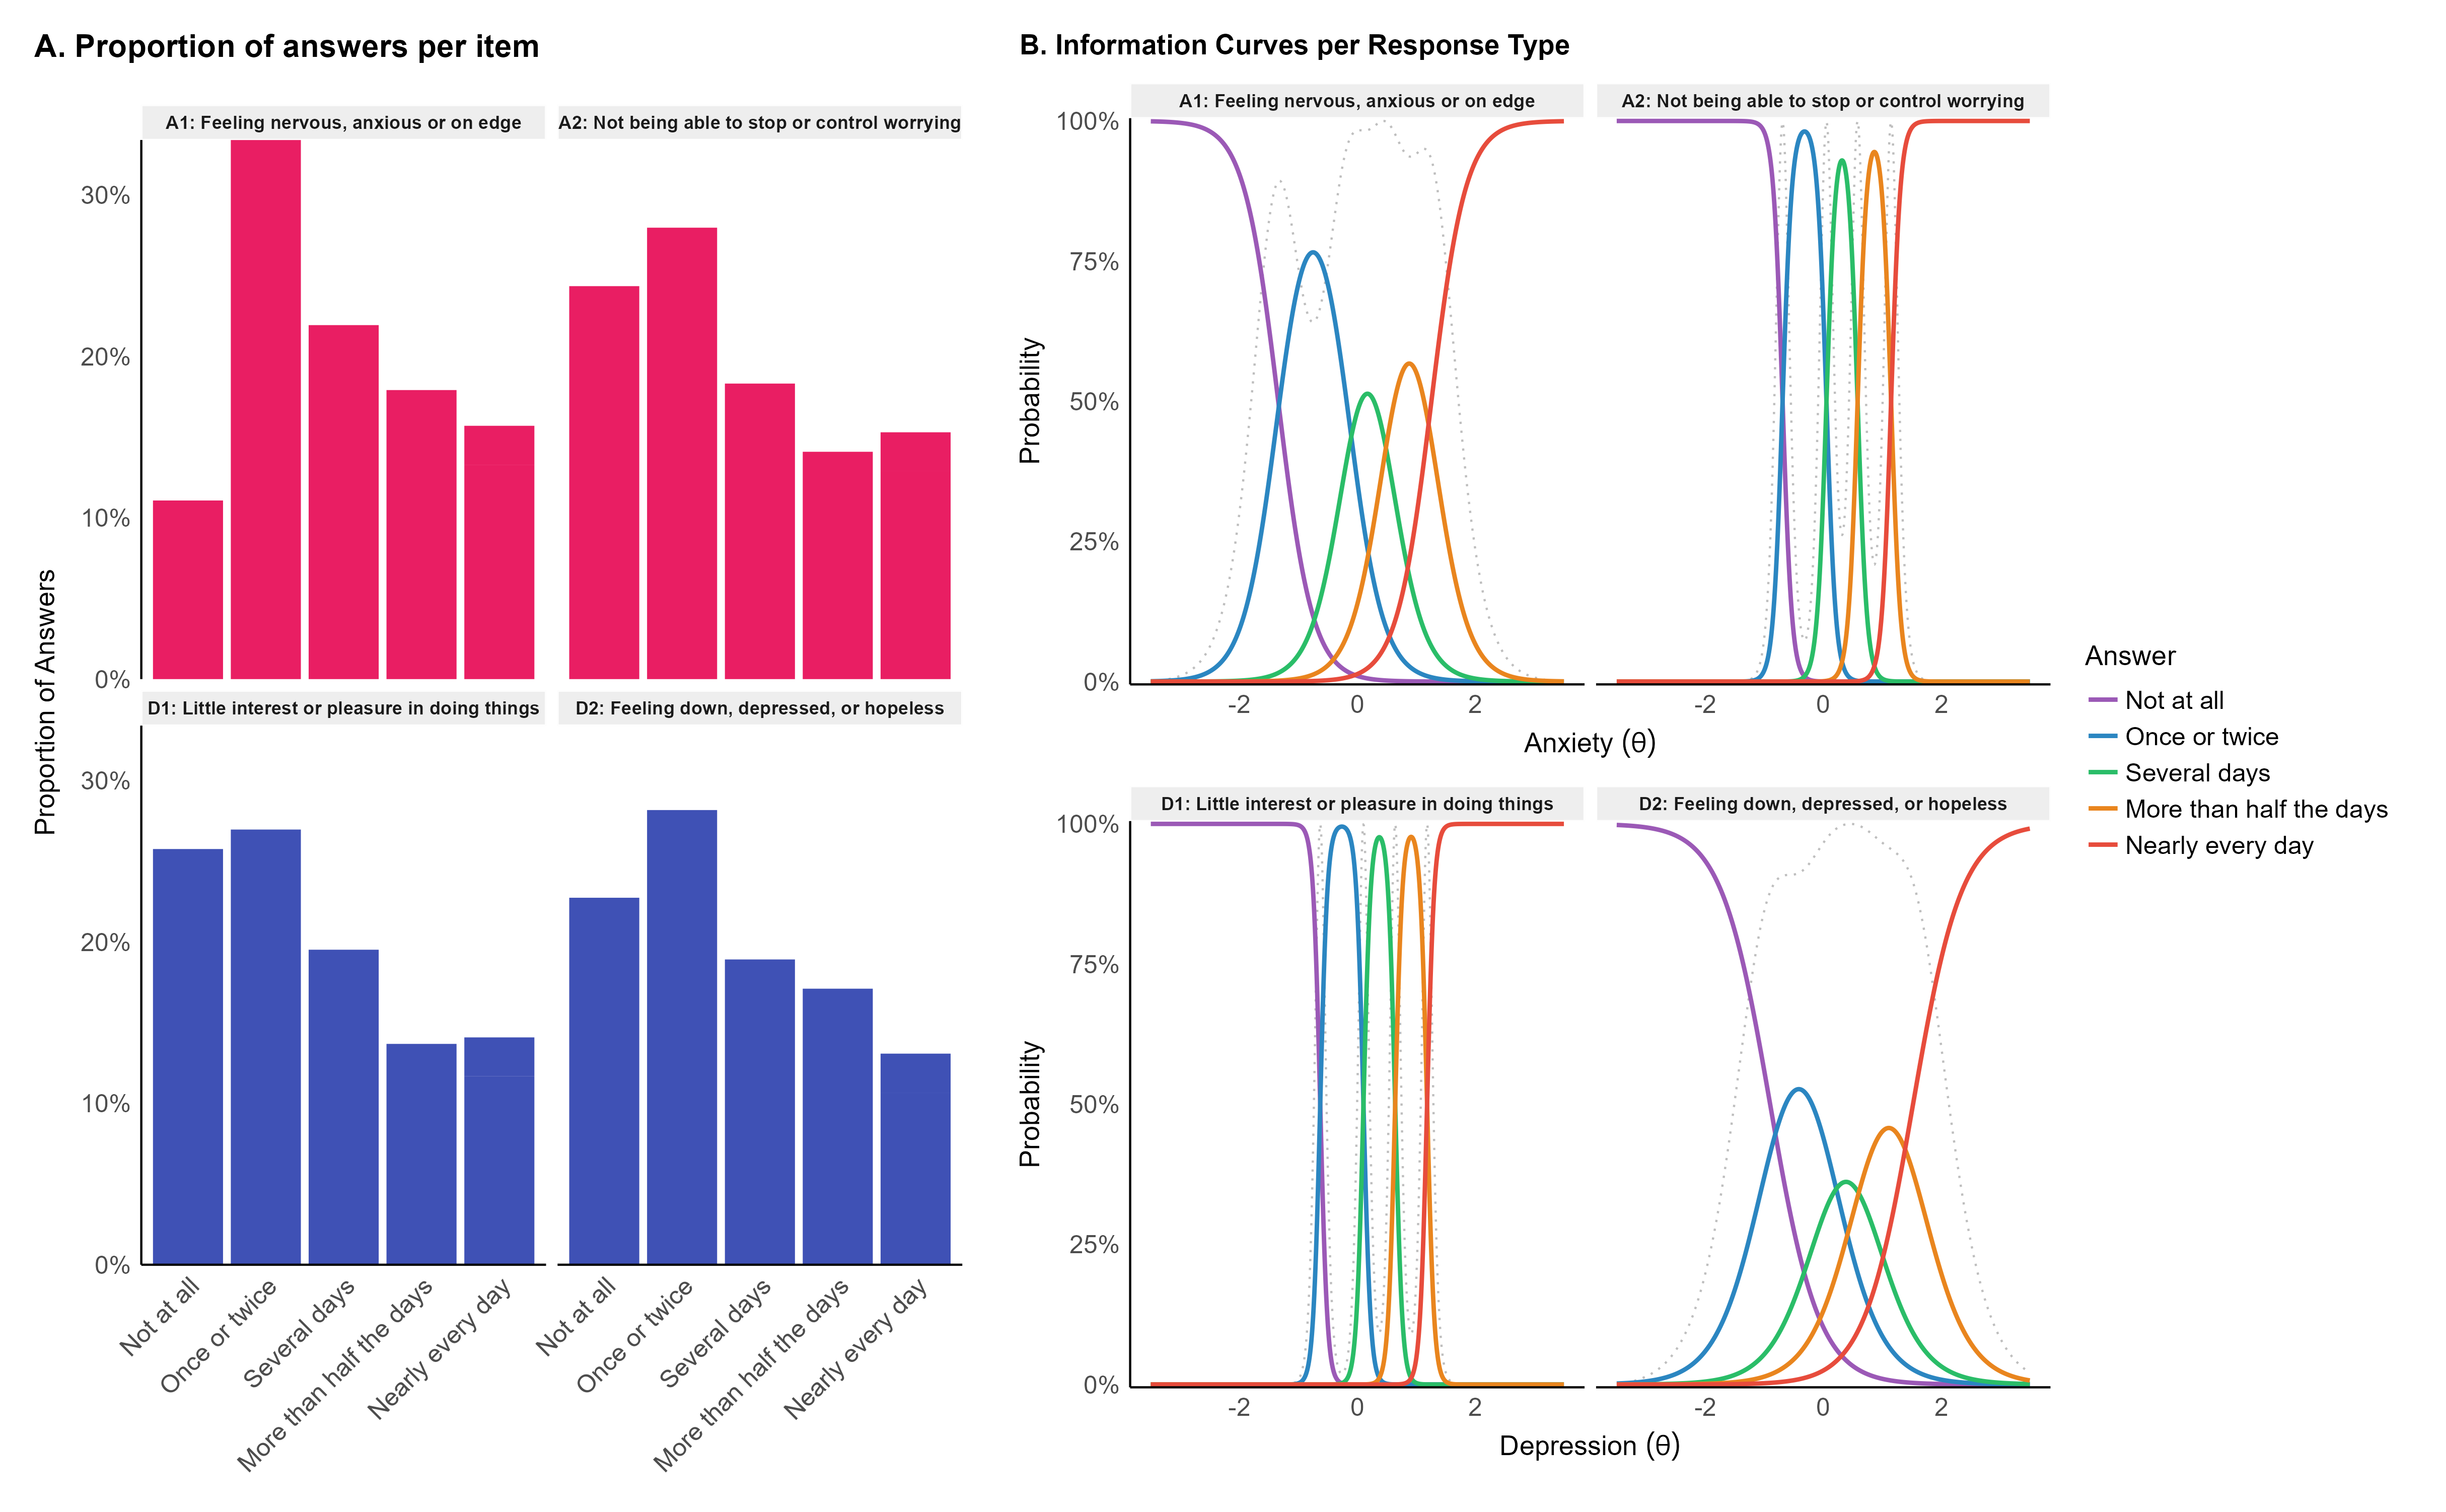
\includegraphics[width=1\linewidth]{../figures/figure1} \caption{A. Proportion of answers of each type. B. Item Information Curves from IRT showing the coverage by each item and response of the latent dimension. Typically, an optimally informative item would display a large coverage over theta, with each response presenting a narrow coverage (high discrimination between different levels).}\label{fig:unnamed-chunk-2}
\end{figure}

\hypertarget{scoring}{%
\subsection{Scoring}\label{scoring}}

We propose two types of scoring procedures. The first aims at
minimally disrupting the original scale and making its scores comparable, enabling comparisons across studies and the usage of developed cut-offs and norms. We suggest to score the new option, ``Once or twice'', as 0.5, occupying the middle space between 0 and 1 (preserving this way the total score range of 0 - 8 per dimension).

The second scoring method we propose takes into account the non-linear spacing between responses, as indicated by the peak of their measurement information. To develop it, we found for each dimension the lower and higher value of the latent trait \(\theta\) for which the probability lower and higher probability of identification is 95\%. We considered these points at 0 and 1, and normalized the location of the peaks of each response in between.

To illustrate, a person answering ``Several days'' and ``Once or twice'' ro the first and second item of the anxiety subscale would have a score of 1.5 (1 + 0.5 following the basic scoring) and a normalized score of 0.50 (\((0.56 + 0.45) / 2\)).

\begin{figure}
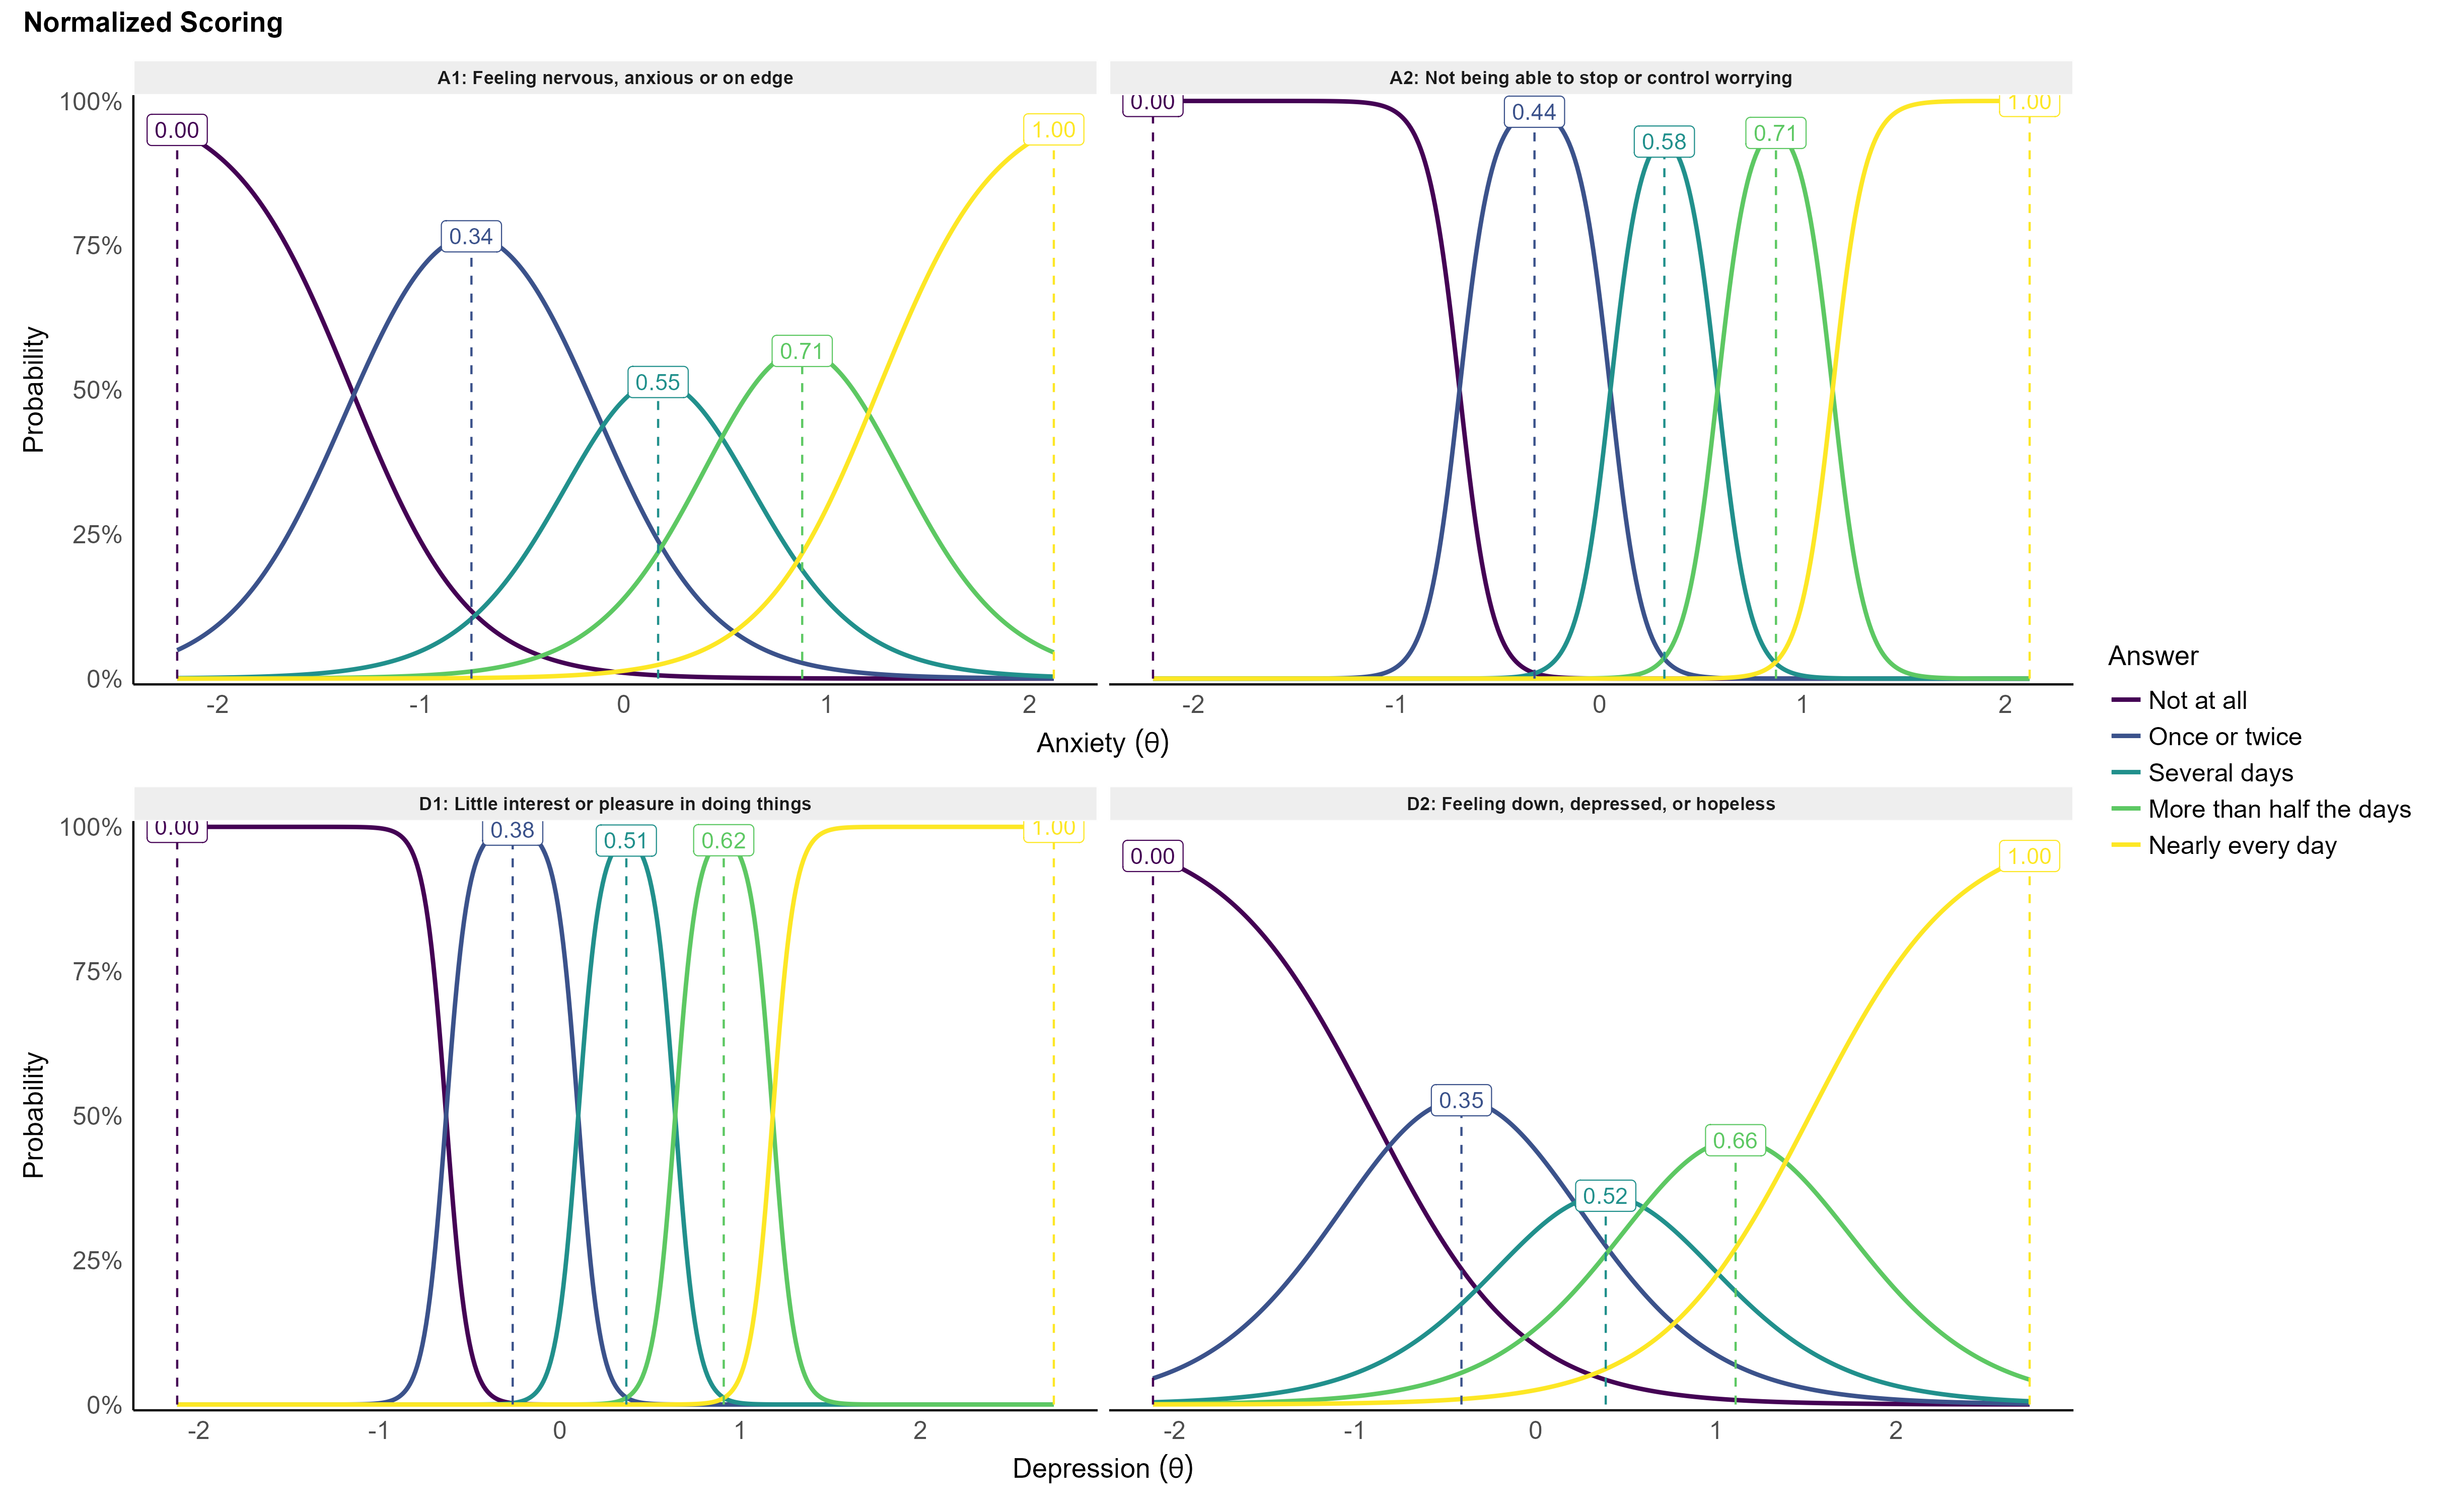
\includegraphics[width=1\linewidth]{../figures/figure2} \caption{Normalized scoring of the items taking into account the non-linear spacing between responses (based on the peak of their measurement information).}\label{fig:unnamed-chunk-3}
\end{figure}

\begin{table}[tbp]

\begin{center}
\begin{threeparttable}

\caption{\label{tab:unnamed-chunk-4}Refined Patient Health Questionnaire-4 (PHQ-4R). The instructions are "Over the last 2 weeks, how often have you been bothered by the following problems?". The 0.5 scoring is introduced to preserve the compatibility with the original version, and enables to use its norms and cut-offs. The normalized scoring takes into account the non-linear spacing between item responses.}

\scriptsize{

\begin{tabular}{lllll}
\toprule
Facet & Item & Response & Basic Scoring & Normalized Scoring\\
\midrule
\textbf{Anxiety} & Feeling nervous, anxious or on edge & \textit{Not at all} & 0 & 0\\
 &  & \textit{Once or twice} & 0.5 & 0.5\\
 &  & \textit{Several days} & 1 & 0.7\\
 &  & \textit{More than half the days} & 2 & 0.8\\
 &  & \textit{Nearly every day} & 3 & 1\\ \midrule
 & Not being able to stop or control worrying & \textit{Not at all} & 0 & 0\\
 &  & \textit{Once or twice} & 0.5 & 0.5\\
 &  & \textit{Several days} & 1 & 0.7\\
 &  & \textit{More than half the days} & 2 & 0.8\\
 &  & \textit{Nearly every day} & 3 & 1\\ \midrule
\textbf{Depression} & Little interest or pleasure in doing things & \textit{Not at all} & 0 & 0\\
 &  & \textit{Once or twice} & 0.5 & 0.5\\
 &  & \textit{Several days} & 1 & 0.7\\
 &  & \textit{More than half the days} & 2 & 0.8\\
 &  & \textit{Nearly every day} & 3 & 1\\ \midrule
 & Feeling down, depressed, or hopeless & \textit{Not at all} & 0 & 0\\
 &  & \textit{Once or twice} & 0.5 & 0.5\\
 &  & \textit{Several days} & 1 & 0.7\\
 &  & \textit{More than half the days} & 2 & 0.8\\
 &  & \textit{Nearly every day} & 3 & 1\\
\bottomrule
\end{tabular}

}

\end{threeparttable}
\end{center}

\end{table}

\hypertarget{discussion}{%
\section{Discussion}\label{discussion}}

The objective of this study was to test the introduction of a ``Once or twice'' response option to the PHQ-4 to make it more sensitive to milder fluctuations. The fact that this new response option was the most prevalent is in itself evidence for its usefulness, and IRT analysis further revealed how this response captures with precision a unique portion of anxiety and depression. Our results suggest that adding this option response increases the scale's potential to discriminate average mood levels (which are superior to zero) from lower-end extremes (the true zero).

\hypertarget{data-availability}{%
\section{Data Availability}\label{data-availability}}

The dataset analysed during the current study are available in the GitHub repository \url{https://github.com/DominiqueMakowski/PHQ4R}

\hypertarget{funding}{%
\section{Funding}\label{funding}}

This work was supported by the Presidential Postdoctoral Fellowship Grant (NTU-PPF-2020-10014) from Nanyang Technological University (awarded to DM).

\newpage

\hypertarget{references}{%
\section{References}\label{references}}

\hypertarget{refs}{}
\begin{CSLReferences}{1}{0}
\leavevmode\vadjust pre{\hypertarget{ref-christodoulaki2022validation}{}}%
Christodoulaki, A., Baralou, V., Konstantakopoulos, G., \& Touloumi, G. (2022). Validation of the patient health questionnaire-4 (PHQ-4) to screen for depression and anxiety in the greek general population. \emph{Journal of Psychosomatic Research}, \emph{160}, 110970.

\leavevmode\vadjust pre{\hypertarget{ref-dobson1979equidistant}{}}%
Dobson, K. S., \& Mothersill, K. J. (1979). Equidistant categorical labels for construction of likert-type scales. \emph{Perceptual and Motor Skills}, \emph{49}(2), 575--580.

\leavevmode\vadjust pre{\hypertarget{ref-hajek2020prevalence}{}}%
Hajek, A., \& König, H.-H. (2020). Prevalence and correlates of individuals screening positive for depression and anxiety on the phq-4 in the german general population: Findings from the nationally representative german socio-economic panel (GSOEP). \emph{International Journal of Environmental Research and Public Health}, \emph{17}(21), 7865.

\leavevmode\vadjust pre{\hypertarget{ref-kroenke2009ultra}{}}%
Kroenke, K., Spitzer, R. L., Williams, J. B., \& Löwe, B. (2009). An ultra-brief screening scale for anxiety and depression: The PHQ--4. \emph{Psychosomatics}, \emph{50}(6), 613--621.

\leavevmode\vadjust pre{\hypertarget{ref-lowe20104}{}}%
Löwe, B., Wahl, I., Rose, M., Spitzer, C., Glaesmer, H., Wingenfeld, K., Schneider, A., \& Brähler, E. (2010). A 4-item measure of depression and anxiety: Validation and standardization of the patient health questionnaire-4 (PHQ-4) in the general population. \emph{Journal of Affective Disorders}, \emph{122}(1-2), 86--95.

\leavevmode\vadjust pre{\hypertarget{ref-materu2020psychometric}{}}%
Materu, J., Kuringe, E., Nyato, D., Galishi, A., Mwanamsangu, A., Katebalila, M., Shao, A., Changalucha, J., Nnko, S., \& Wambura, M. (2020). The psychometric properties of PHQ-4 anxiety and depression screening scale among out of school adolescent girls and young women in tanzania: A cross-sectional study. \emph{BMC Psychiatry}, \emph{20}(1), 1--8.

\leavevmode\vadjust pre{\hypertarget{ref-maurer2018depression}{}}%
Maurer, D. M., Raymond, T. J., \& Davis, B. N. (2018). Depression: Screening and diagnosis. \emph{American Family Physician}, \emph{98}(8), 508--515.

\leavevmode\vadjust pre{\hypertarget{ref-mendoza2022factor}{}}%
Mendoza, N. B., Frondozo, C. E., Dizon, J. I. W. T., \& Buenconsejo, J. U. (2022). The factor structure and measurement invariance of the PHQ-4 and the prevalence of depression and anxiety in a southeast asian context amid the COVID-19 pandemic. \emph{Current Psychology}, 1--10.

\leavevmode\vadjust pre{\hypertarget{ref-samejima1997graded}{}}%
Samejima, F. (1997). Graded response model. In \emph{Handbook of modern item response theory} (pp. 85--100). Springer.

\end{CSLReferences}


\clearpage
\renewcommand{\listfigurename}{Figure captions}


\end{document}
